\chapter{Systemmodels}
\label{ch:sysmodels}

\section{System architecture}
\label{sec:sysarchitecture}
The specified criteria demand for a minimalist user interface and little to no bidirectional data flow within the application. As the main focus of this project is collecting, processing and finally storing data, the applied architecture will be a pipeline architecture.

\subsection{Basic Pipeline}
\label{sec:sm_basicpipe}
The traditional pipeline architecture refers to a process being split up into several sequential steps, ideally with data buffers in between those, which will be able to independently and possibly asynchronously perform a specific transformation on their data input. The resulting data will then be provided as output for the subsequent step. This works especially well in a scenario where only an unidirectional data flow is required.
\begin{figure}[h!]
  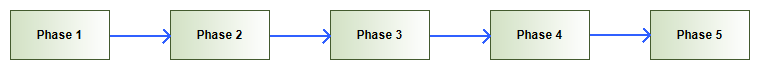
\includegraphics[width=1.00\textwidth]{resources/simplepipeline.png}
  \centering
  \caption{A simple pipeline model}
  \label{fig:sm_basicpipe}
\end{figure}

\subsection{The extended pipeline}
\label{sec:sm_extpipe}
In this project, the basic pipeline is an insufficient model, as the initial input data will have to be gathered at several, mostly independent places. The \gls{browser} module (see \specref{FS440} to \specref{FS449}) will only capture \gls{browser} \glspl{event}, the window management \gls{module} (see \specref{FS400} to \specref{FS404}) cannot also provide the keyboard input etc. In order to solidify all the collected \glspl{event}, the extended pipeline allows for a single processing step to accept input from multiple sources by utilizing the transforming modules as mentioned in \ref{transforming-module}. The result is a tree-structure where the \gls{event}-data strictly flows from the leafs towards the root, the root being the core application (see \ref{sec:func_core}).
\begin{figure}[h!]
  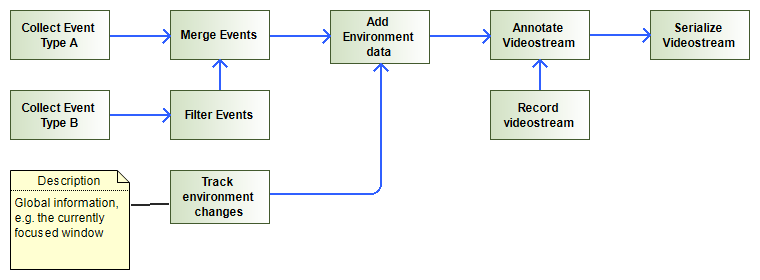
\includegraphics[width=1.00\textwidth]{resources/extendedpipeline.png}
  \centering
  \caption{An extended pipeline model}
  \label{fig:sm_extpipe}
\end{figure}

\subsection{Module types}
\label{sec:module-types}


The application needs to provide three different types of \glspl{module}:
\begin{itemize}
        \item Collecting \glspl{module}\label{collecting-module}\\\Glspl{module} which accept no input from other \glspl{module} and generate one or more \glspl{event} as output.
        \item Transforming \glspl{module}\label{transforming-module}\\\Glspl{module} which accept one or more \glspl{event} as input from other \glspl{module} and generate one or more \glspl{event} as output.
        \item Discarding \glspl{module}\label{discarding-module}\\\Glspl{module} which accept one or more \glspl{event} as input from other \glspl{module} and output no \glspl{event}.
\end{itemize}

%\section{Object models}
%%we might not want to specify object models yet

\newpage %%formatting, can potentially be removed later
\section{Dynamic model} %%change to models should addtional charts be added
\label{sec:sm_dynamic_models}
The following figure shows an example of how the application could deal with a \gls{user} clicking on an element in their \gls{browser}. The actual flow might differ based on available modules and rule configuration.
\begin{figure}[H]
  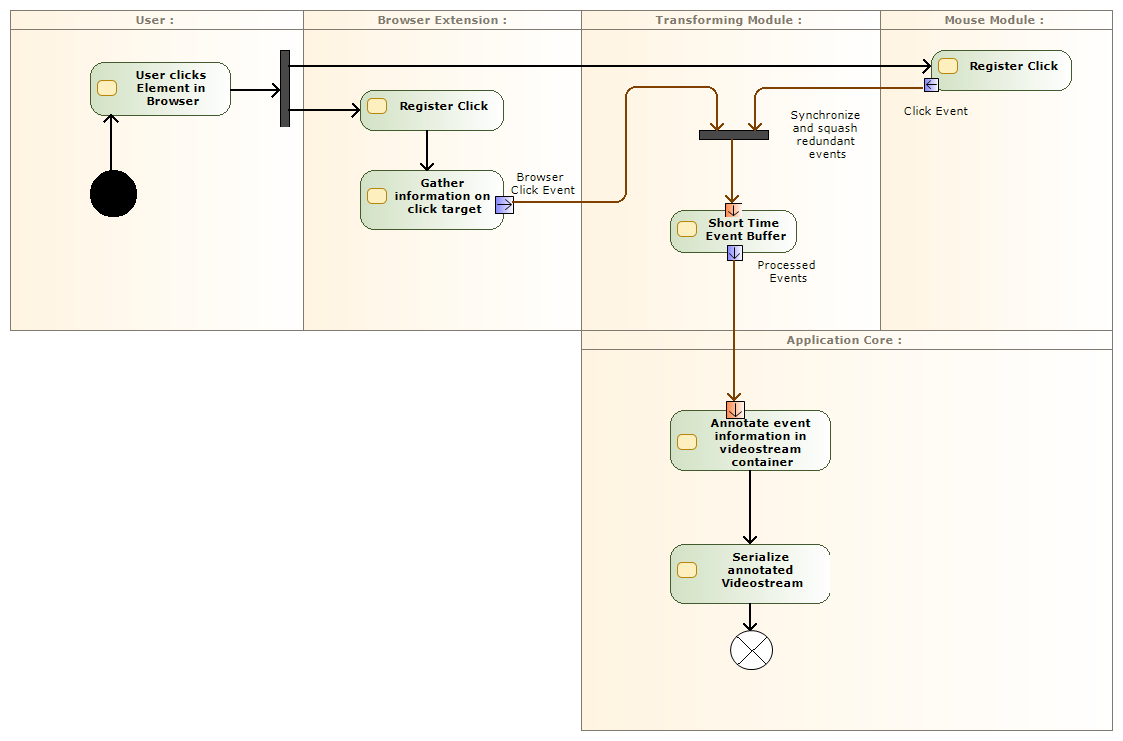
\includegraphics[width=1.00\textwidth]{resources/clickactivity.png}
  \centering
  \caption{User-Click sample activity chart}
  \label{fig:sm_clickactivity}
\end{figure}
\newpage %% for formatting
\section{User Interface}
\label{sec:sm_userinterface}
The \gls{user}-interface is intentionally minimal as the \glspl{user} should not be disrupted during their usual work-routine. The following figures show drafts and therefore do not represent the final product.

\begin{figure}[H]
  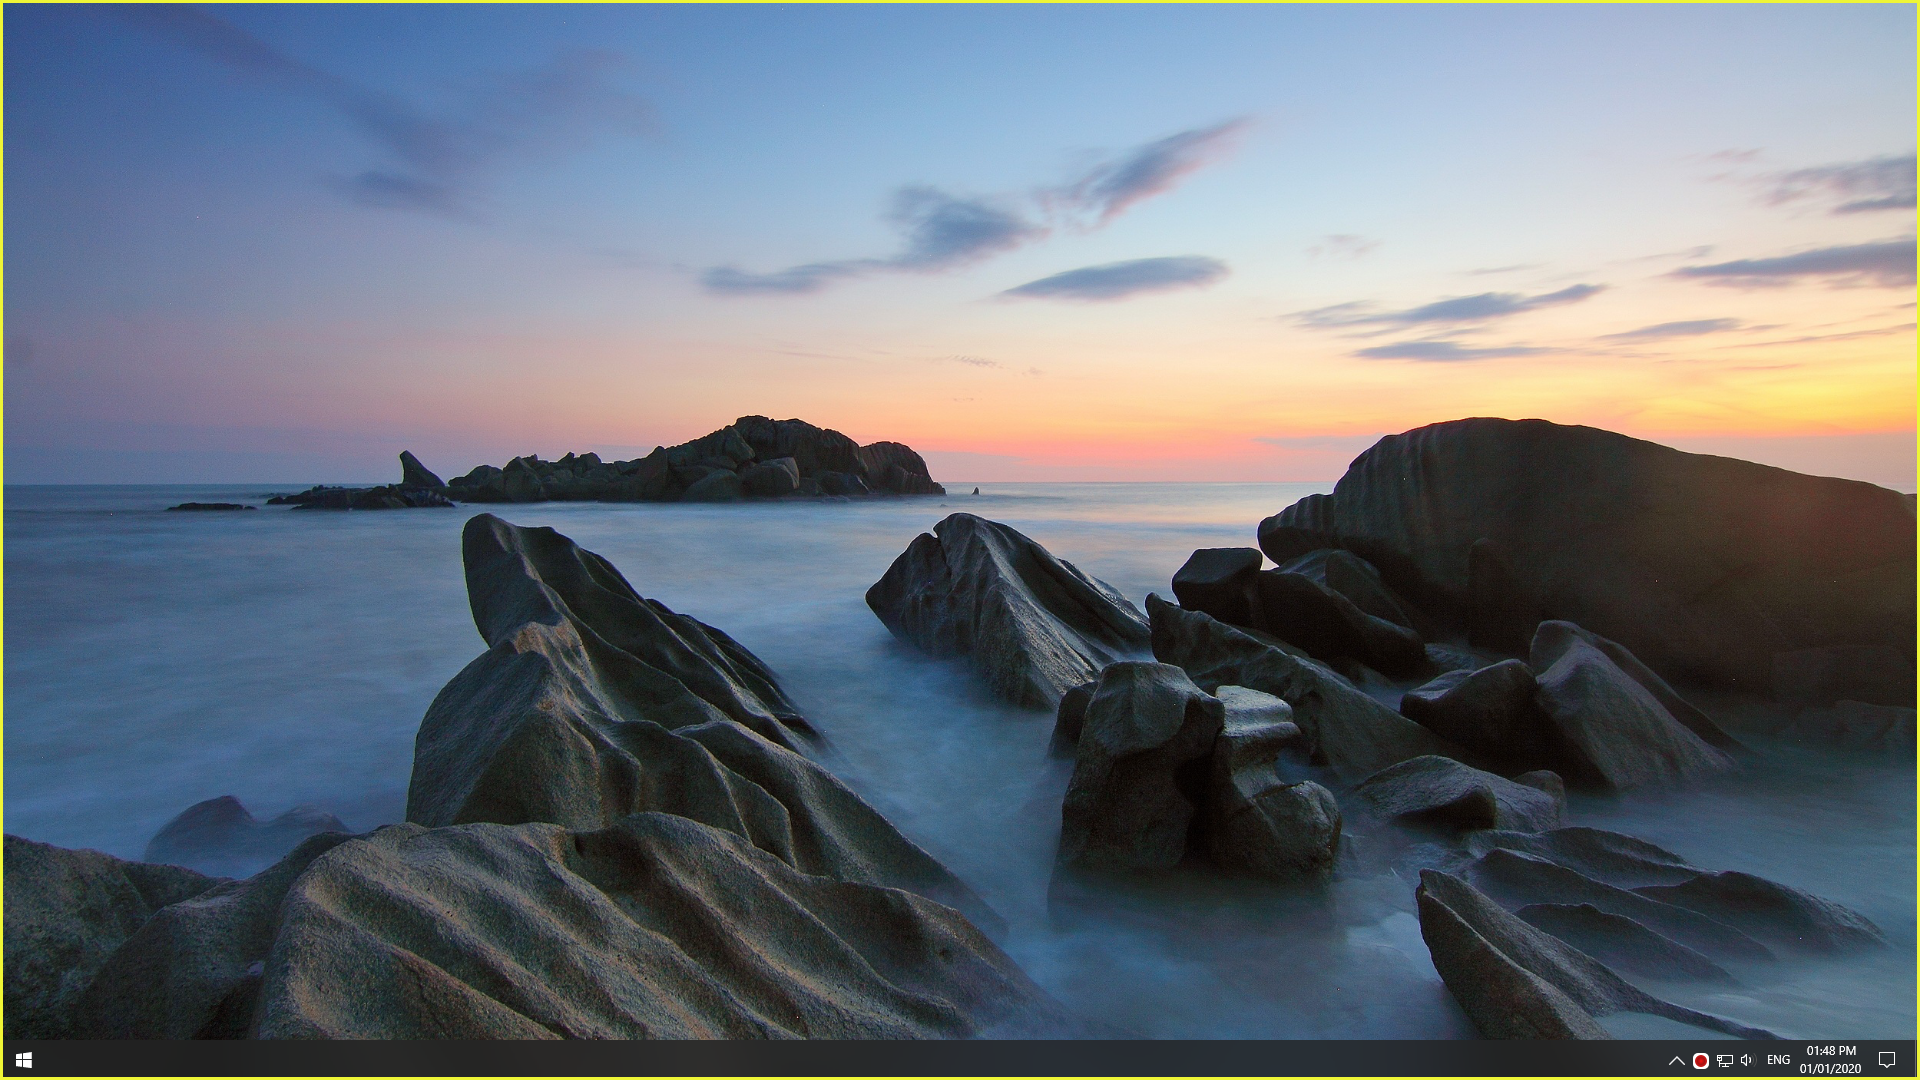
\includegraphics[width=1.00\textwidth]{resources/ui_recording.png}
  \centering
  \caption{A running \gls{session} recording is indicated by a yellow border.}
  \label{fig:sm_ui_recordindicator}
\end{figure}
\begin{figure}[H]
  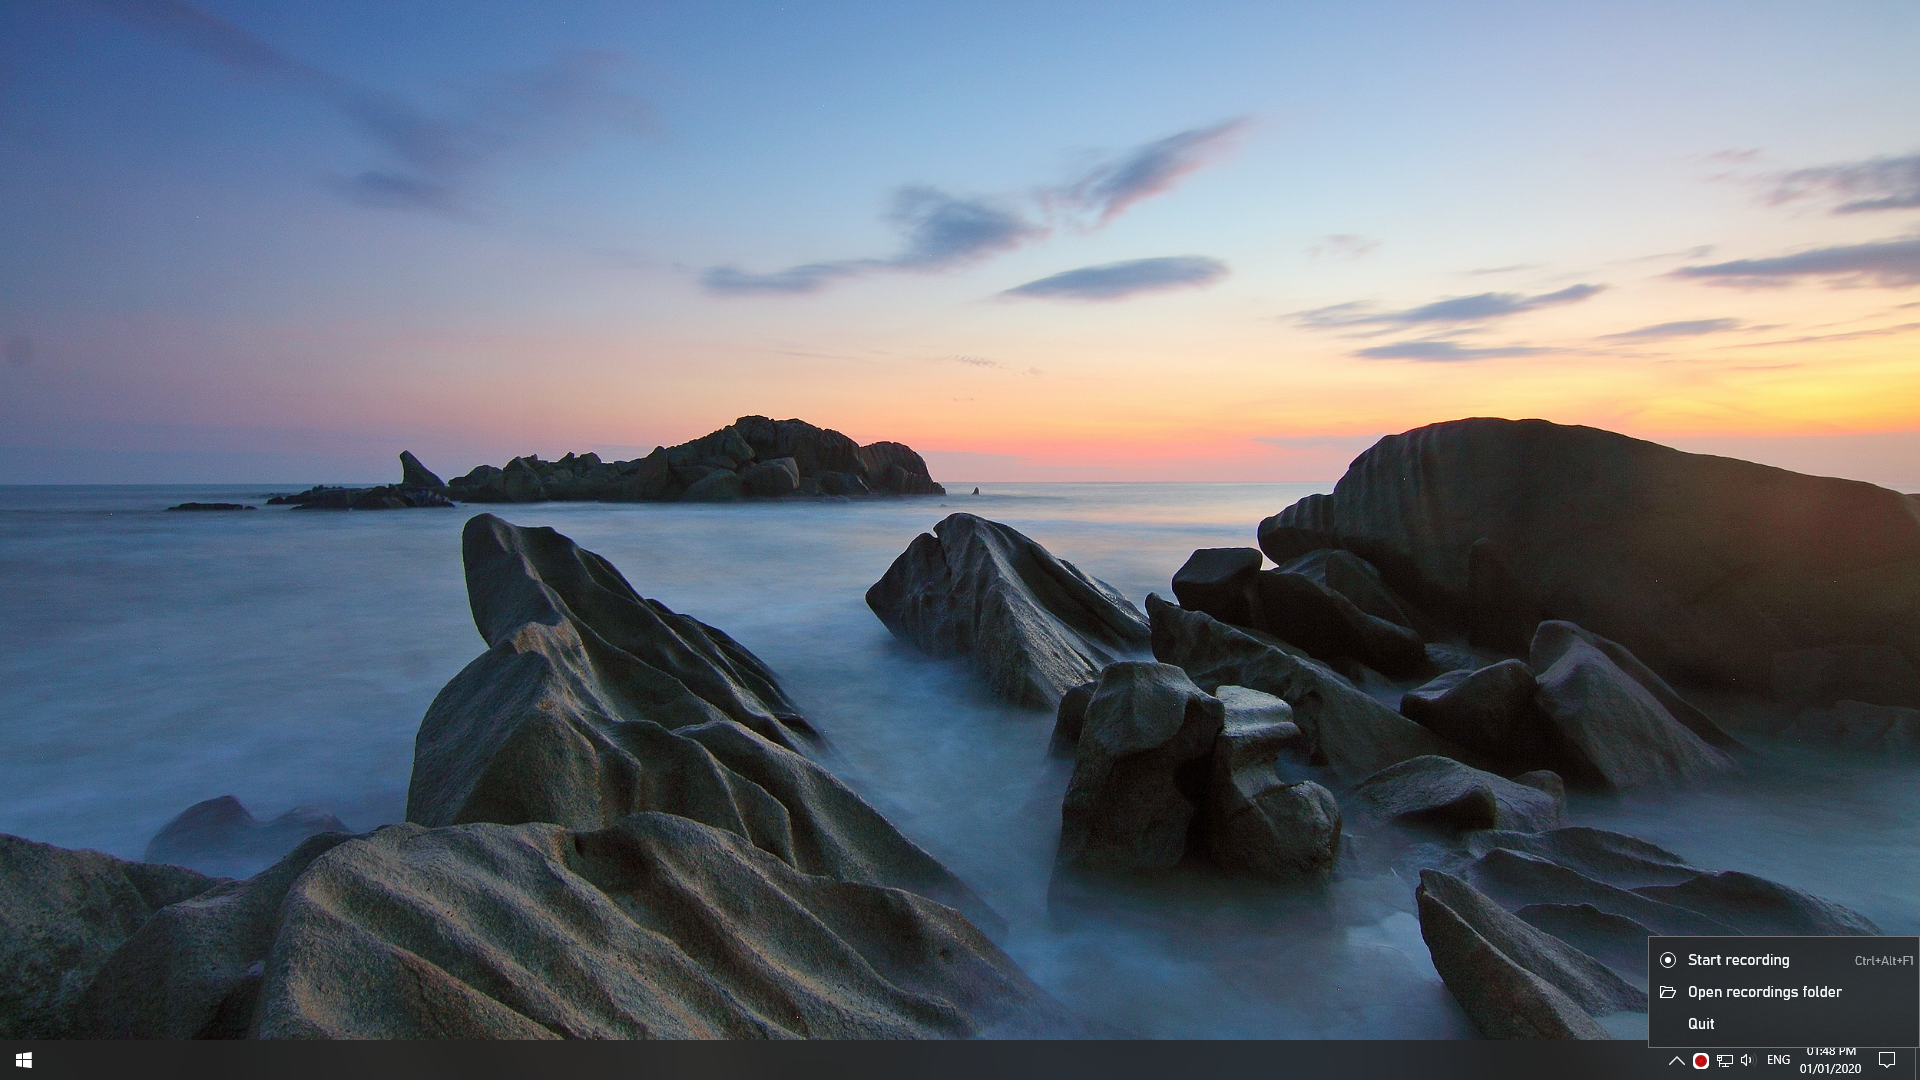
\includegraphics[width=0.5\textwidth, trim={50cm 0 0 25cm},clip]{resources/ui_inactive_tray.png}
  \centering
  \caption{The start/stop recording features may be quickly accessed by clicking on the tray icon (represented by the red dot).}
  \label{fig:sm_ui_trayicon}
\end{figure}
\begin{figure}[H]
  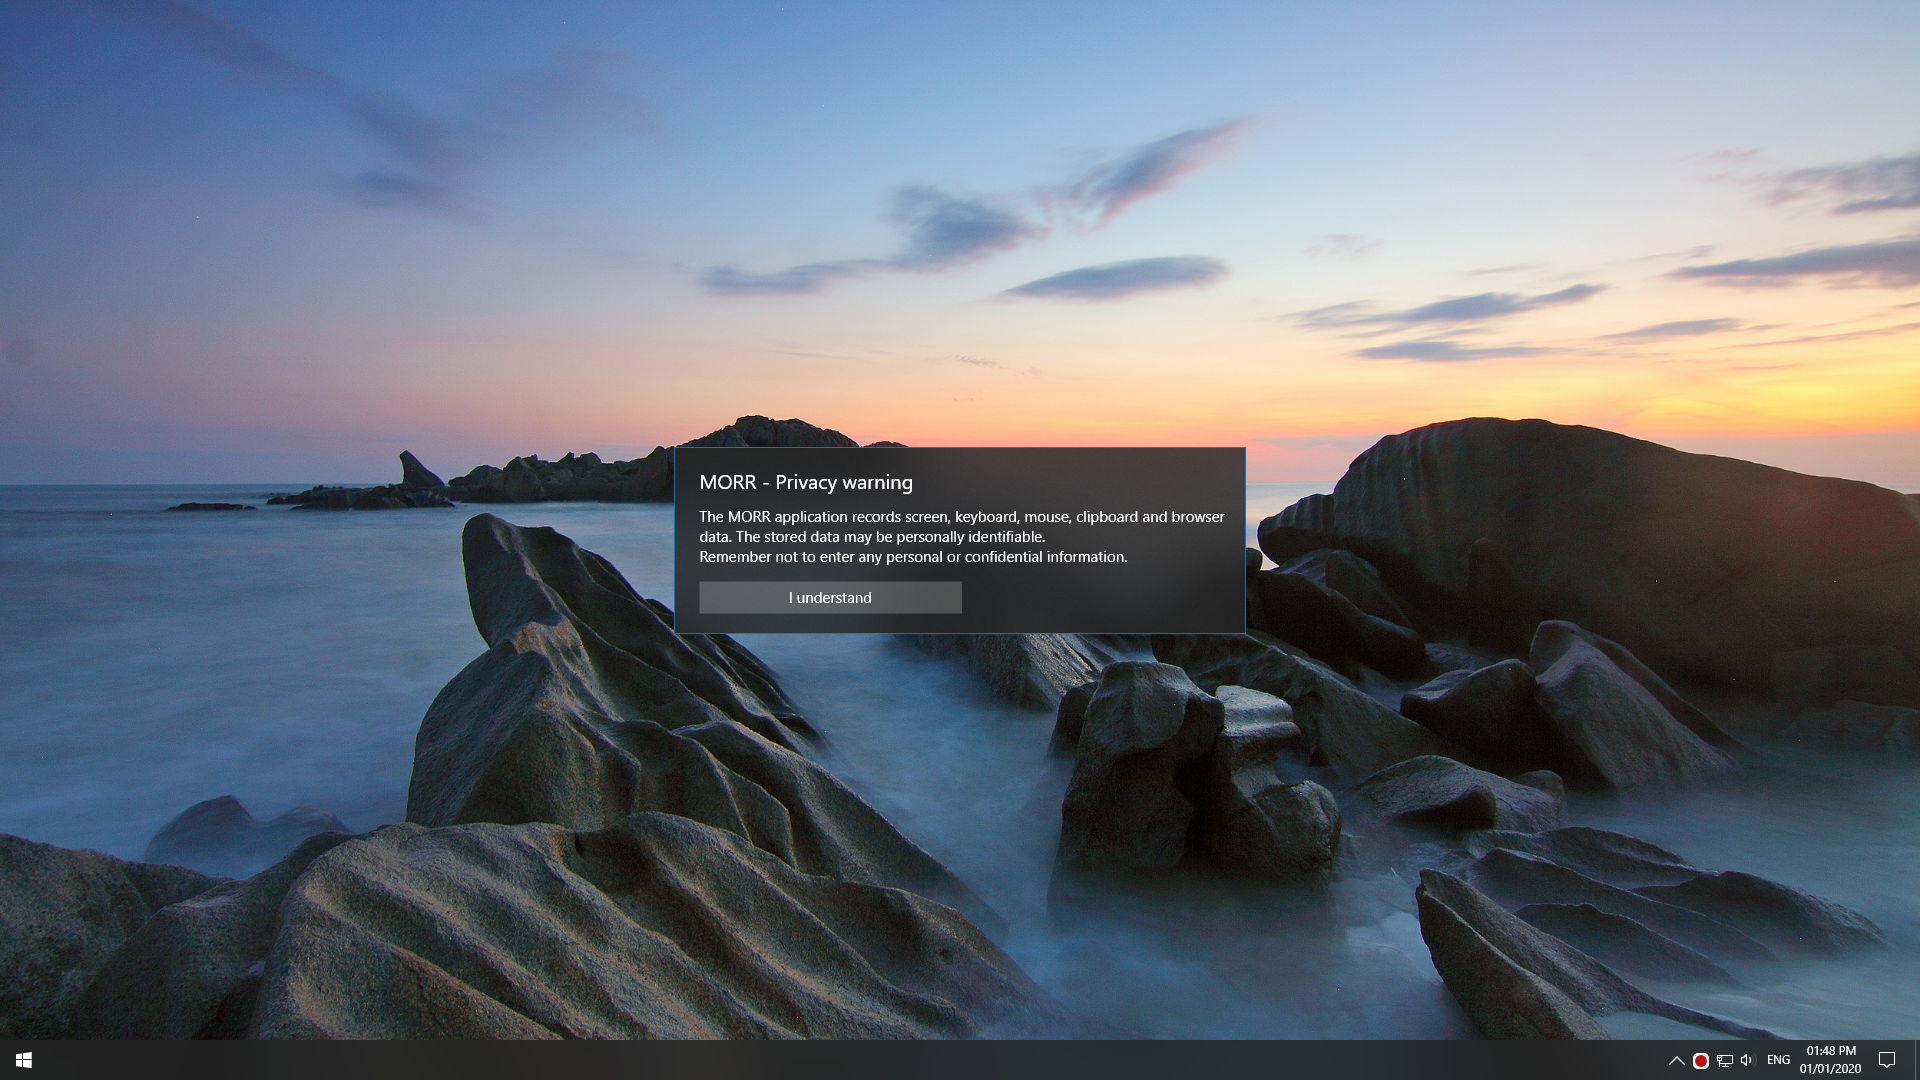
\includegraphics[width=0.8\textwidth, trim={20cm 10cm 20cm 10cm}, clip]{resources/ui_privacy_warning.png}
  \centering
  \caption{The privacy warning appears when a recording is started.}
  \label{fig:sm_ui_privacy}
\end{figure}
\begin{figure}[H]
  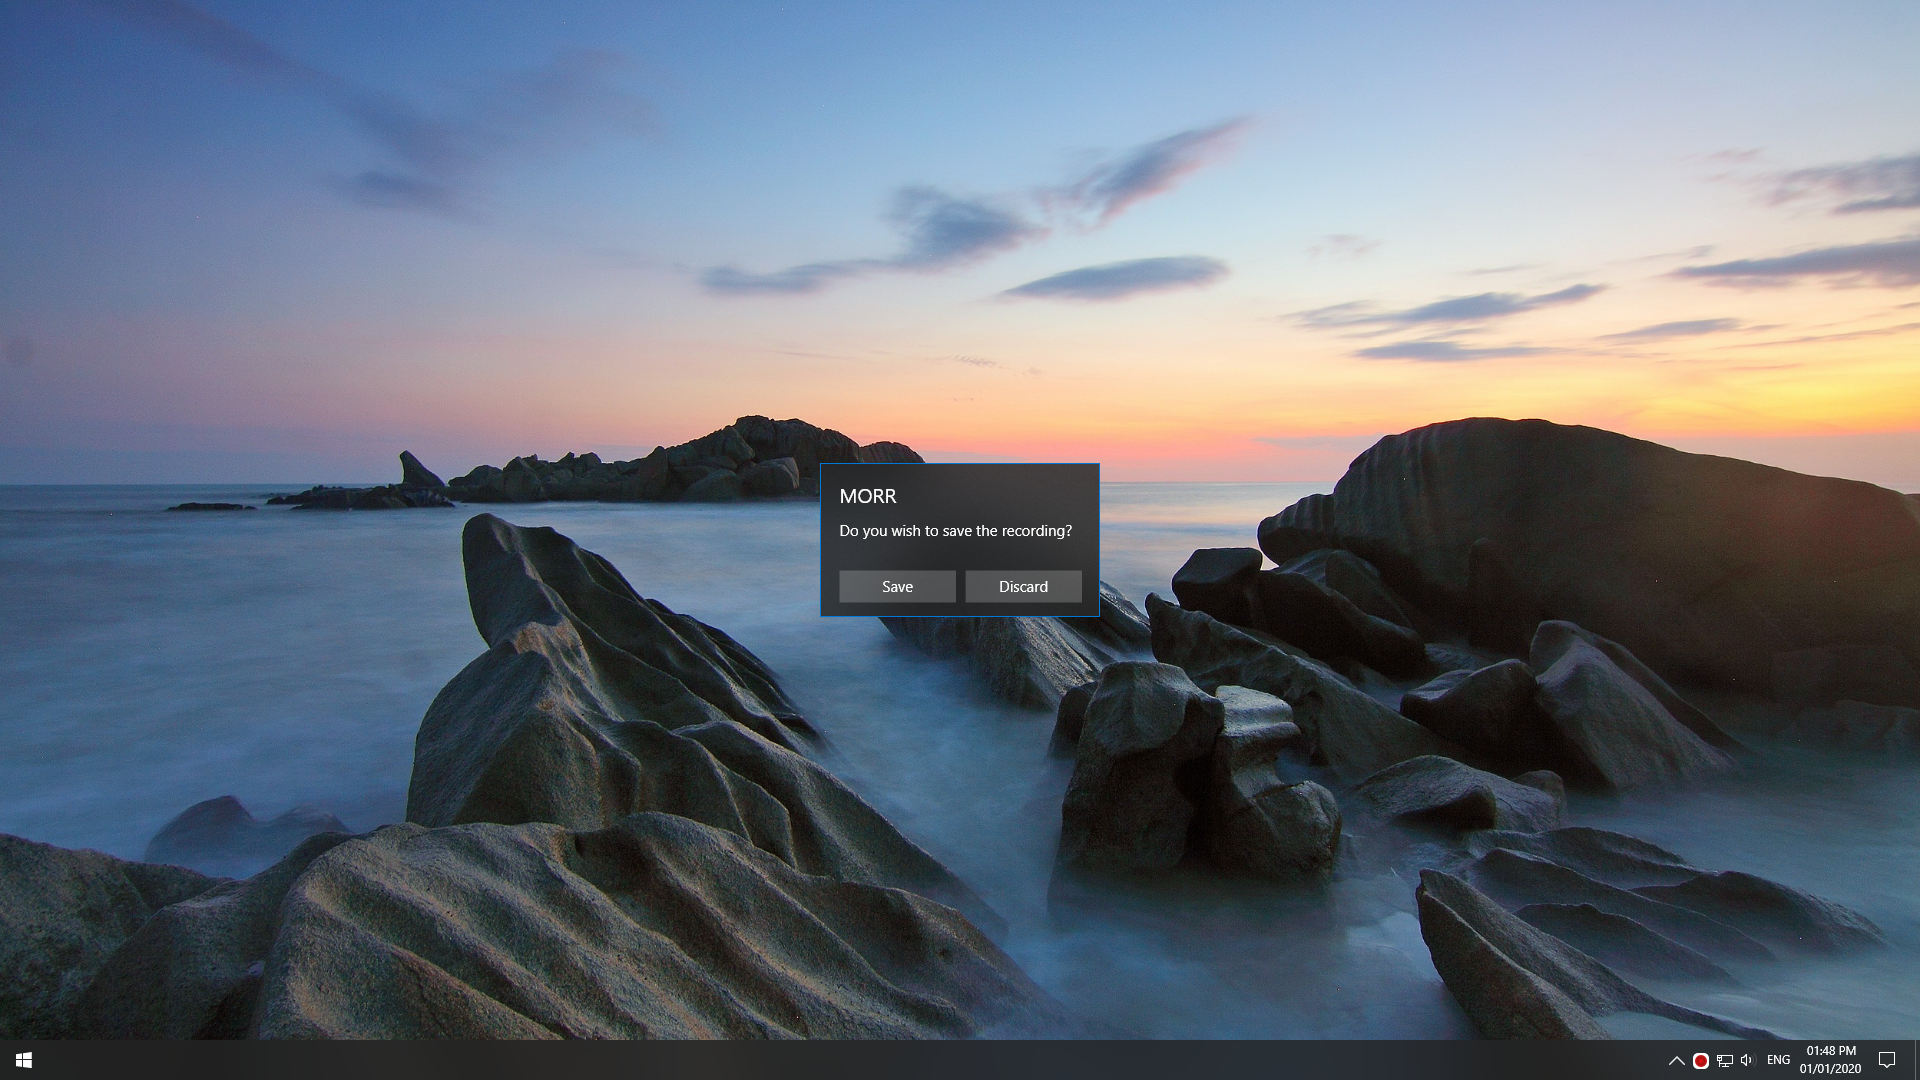
\includegraphics[width=0.8\textwidth, trim={20cm 10cm 20cm 10cm}, clip]{resources/ui_save_dialogue.png}
  \centering
  \caption{The save dialog appears when a recording is stopped.}
  \label{fig:sm_ui_saving}
\end{figure}

\subsection{Data extraction}
\label{sec:sm_extraction}
The \glspl{scientist} will be able to extract \gls{event}-information from the video container by utilizing an API (application programming interface) which will be supplied together with the application. Additionally, the application will be bundled with a commandline-tool which allows for extraction of the \gls{event}-data into the common CSV-format (comma-separated values). See also \specref{FS330}.